\documentclass[final,hyperref={pdfpagelabels=false}]{beamer}
\mode<presentation>{\usetheme{Lankton}}
\boldmath
\usepackage{times}
\usepackage{ragged2e} 
\usepackage{caption}
\usepackage{tabularx}
\usepackage{graphicx}
\usepackage{subcaption}
\usepackage{amsmath,amsthm, amssymb, latexsym}
\usepackage[english]{babel}
\usepackage[latin1]{inputenc}
\usepackage{graphicx}
\graphicspath{{figures/}}
\setbeamertemplate{caption}[numbered]
\usepackage[orientation=landscape,size=a1,scale=1]{beamerposter}

\title{SyntenyFinder: A Synteny Blocks Generation and Genome Comparison Tool}
\author{Ilya Minkin\textsuperscript{1}, Nikolay Vyahhi\textsuperscript{1}, and Son Pham\textsuperscript{2}}
\institute{\textsuperscript{1} St. Petersburg Academic University, St. Petersburg, Russia \\ \textsuperscript{2} University of California, San Diego, USA}

\begin{document}
\begin{frame}{}

\begin{columns}[t]

\begin{column}{0.32\linewidth}

\begin{block}{Introduction} \justifying
Recent advances in sequencing and genome assembling technologies are resulting in many finished genomes.
The comparison of these genomes has been emerging as a powerful tool for genome interpretations.
These tasks often require genomes to be  decomposed to a collection of synteny blocks -- regions of conserved DNA.
\begin{figure}
	\centering
	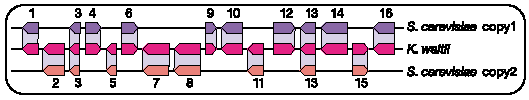
\includegraphics[scale = 2.8]{syntenyBlocks.pdf}
	\small \caption{Rectangles with arrows depict synteny blocks in two yeast genomes (Kellis2004)}
\end{figure}
We propose \textit{SyntenyFinder} -- a tool for finding synteny blocks in genomes represented as nucleotide sequences.
Our approach is based on de Bruijn graph and can be applied to closely related genomes.
\end{block}

\begin{block}{De Bruijn graphs in synteny block mining} \justifying
Given a string \(S\) and a natural number \(k\) we construct the de Bruijn graph \(G(k)\) as follows:

\begin{itemize}
\item For each unique \(k\)-substring add a vertex to \(G(k)\)
\item For each \((k + 1)\)-substring \(w\) in \(S\) add to \(G(k)\) an edge that connects \(k\)-prefix of \(w\) with \(k\)-suffix of \(w\)
\item Label edges with positions of the corresponding \((k + 1)\)-mers
\end{itemize}

\begin{figure}
	\centering
	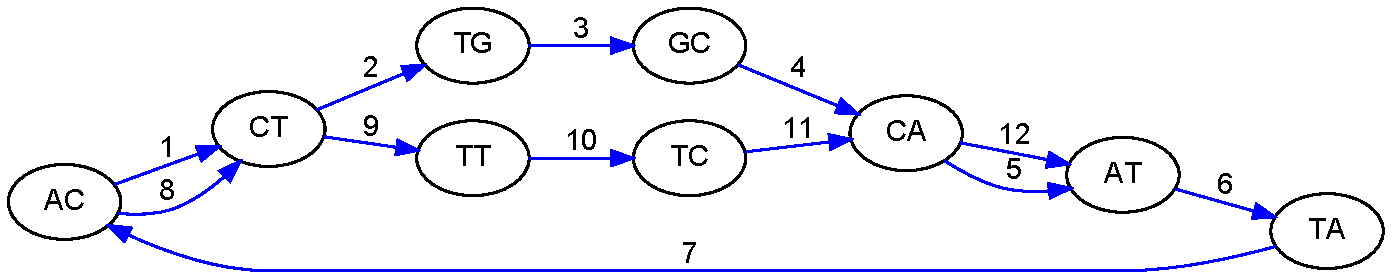
\includegraphics[scale = 0.9]{simpleGraph.pdf}
	\small \caption{De Bruijn graph \(G(2)\) built from string \("ACTGCATACTTCAT"\), bulge indicates a mismatch}
\end{figure}             

In this graph we allow only paths that have consecutive labels on edges.
Graph \(G(k)\) has following properties:

\begin{itemize}
\item Each valid path in the graph spells a substring from \(S\)
\item Non-branching paths in the graph indicate exact repeats in \(S\)
\item Variations in repeats create \textit{bulges} in \(G(k)\)
\item Bulges are formed by two disjoint valid paths with shared ends
\end{itemize}

We remove bulges with size larger than some predefined constant \(\delta\) to obtain long non-branching paths. This process is 
called \textit{simplification}.
\end{block}

\end{column}

\begin{column}{0.32\linewidth}

\begin{block}{Double strandness issue} \justifying
DNA has two strands and synteny blocks can be located on both. 
We address this problem by:
\begin{itemize}
\item Building graphs for both strands separately
\item Labeling edges in these graphs with two different colors
\item Merging two graphs and work with the resulting graph 
\end{itemize}
\end{block}

\begin{block}{SyntenyFinder algorithm} \justifying
Given two numbers \(k\) and \(\delta\) and a set \(S = \lbrace S_{1}, S_{2}, \ldots, S_{n} \rbrace \) of chromosomes 
represented as nucleotide strings, our algorithm works as follows:
\begin{itemize}
\item Concatenate all chromosomes in \(S\) into the supergenome \(\hat{S}\)
\item Construct graph \(G ^ +(k)\) from \(\hat{S}\) and color all its edges \textit{blue}
\item Construct graph \(G ^ -(k)\) from reverse-complementary of \(\hat{S}\) and color all its edges \textit{red}
\item Obtain \(G(k) = G ^ +(k) \cup G ^ -(k)\) 
\item Change \(\hat{S}\) so that \(G(k)\) doesn't contain bulges having size \( < \delta \)
\item Output non-branching paths as synteny blocks
\end{itemize}
At any moment during simplification there is a one-to-one correspondence between the string and the graph -- any changes in \(\hat{S}\) are immediately reflected in \(G(k)\).

We also keep some information on the edges to be able to reconstruct original coordinates of the found synteny blocks.

\begin{figure}
        \begin{subfigure}[a]{1\textwidth}
		\centering
		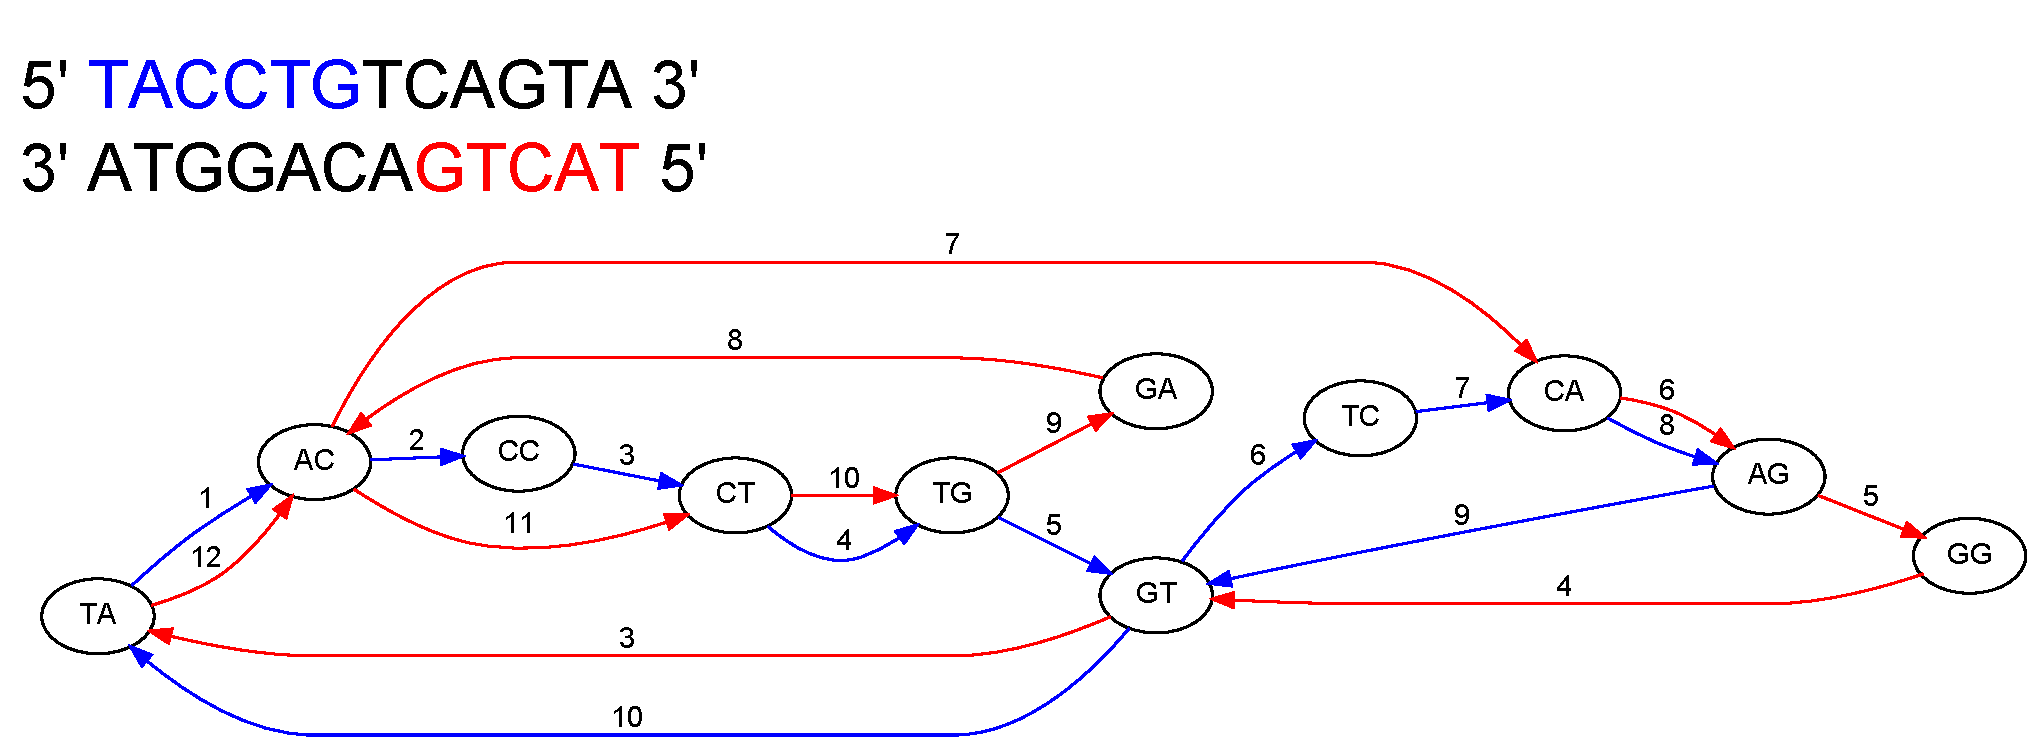
\includegraphics[scale = 1.30]{graph1.pdf}
		\justifying
		\small \caption{Fragment of a two-colored de Bruijn graph, bulge indicates an indel}
		\label{DeBruijnA}
        \end{subfigure}
        \begin{subfigure}[b]{1\textwidth}
		\centering
		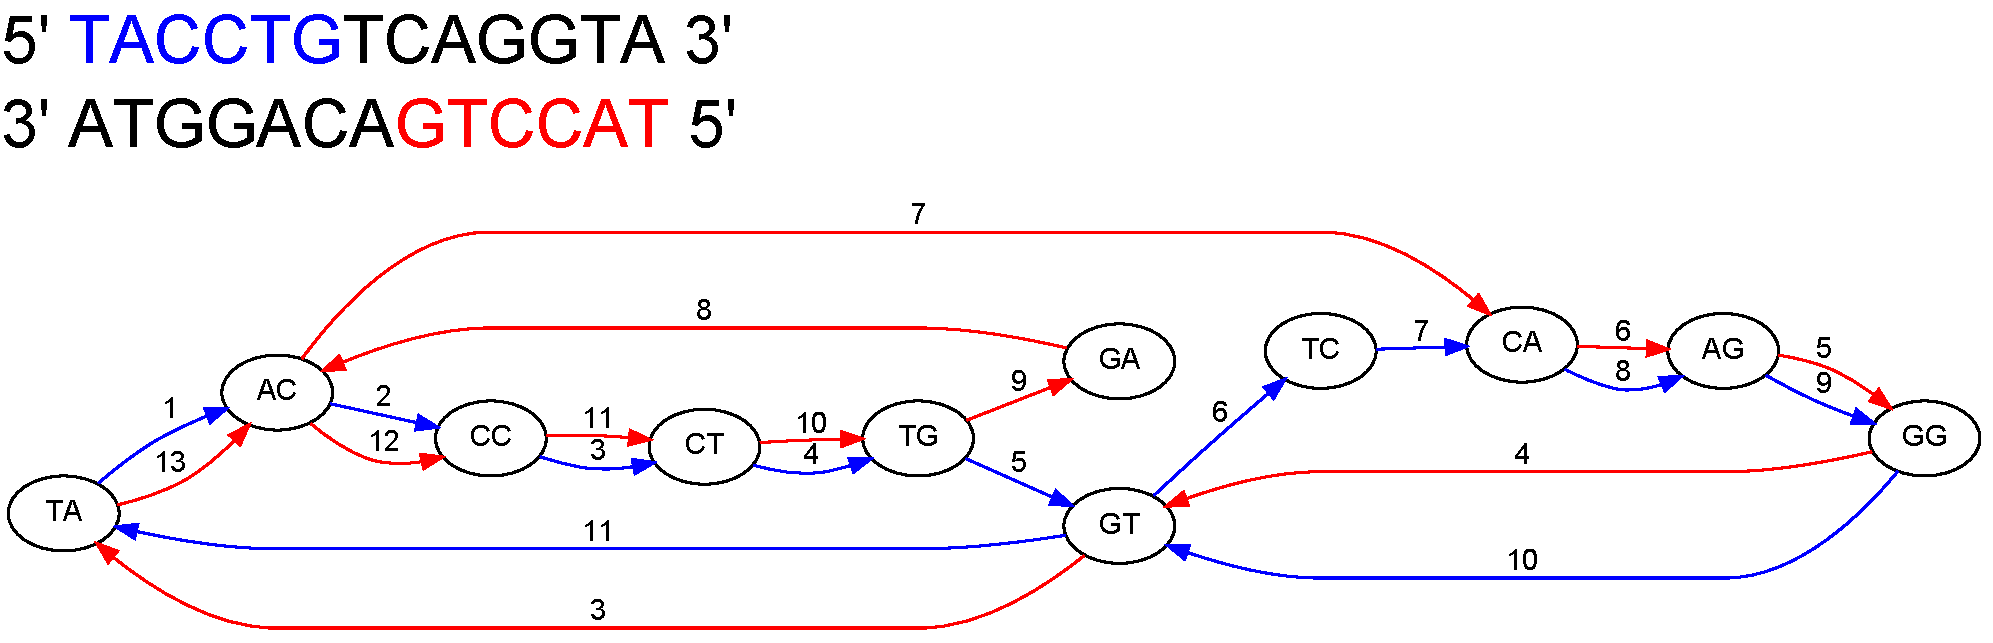
\includegraphics[scale = 1.30]{graph2.pdf}
		\small \caption{Fragment of the same graph after simplification}
		\label{DeBruijnB}
        \end{subfigure}
	\small \caption{Illustration of the bulge removal}
\end{figure}

\end{block}

\end{column}

\begin{column}{0.32\linewidth}

\begin{block}{Results} \justifying
We benchmark SyntenyFinder on two datasets.
\begin{itemize}
\item Four strains of the bacteria \textit{Pseudomonas aeruginosa}
\item Two different yeast species: \textit{K.waltii} and \textit{S. cerevisiae}
\end{itemize}

\begin{table}
\small
\begin{tabularx}{\textwidth}{ | X | X | X | X | X | X | X |}
	\hline
	Dataset & Total size & \(k\) & \(\delta\) & Multiplicity & Count & Coverage\\
	\hline \hline
	Bacteria & 27 MBP & 1000 & 5000 & 4 & 140 & 90\% \\
	\hline
	Yeast    &  23 MBP & 1000 & 20000 & 3 &  270 & 64\% \\
	\hline
\end{tabularx}
\end{table}

For the yeasts we used local alignments from (Kellis2004) to enrich number of common \(k\)-mers in conserved regions.
Our blocks share 80\% of their basepairs with the blocks described in (Kellis2004).
\end{block}

\begin{block}{Discussion} \justifying
SyntenyFinder can be efficiently used for finding synteny blocks in closely related genomes represented as nucleotide sequences. 
Benchmarks show that with some modifications our method can be applied to more distant genomes. Our near plans include:
\begin{itemize}
\item Release version for closely related species
\item Extend SyntenyFinder to a wider range of genomes
\item Incorporate it into genome rearrangements analysis tools
\end{itemize}
\end{block}

\begin{block}{Acknowledgments} \justifying
We would like to thank Pavel Pevzner, Steve O'Brien, Alla Lapidus, Matt Schultz and Dinh Diep for their 
for their help and contributions to many helpful discussions.

This work was supported by the Government of the Russian Federation (grant 11.G34.31.0018)
and the National Institutes of Health (NIH grant 3P41RR024851-02S1).
\end{block}

\begin{block}{References} \justifying
\begin{thebibliography}{10}
\small
\beamertemplatebookbibitems
\bibitem{Kellis2004}
Kellis M, Birren BW, Lander ES
\newblock Proof and evolutionary analysis of ancient genome duplication in the yeast Saccharomyces cerevisiae.
\newblock {\em Nature}, 2004 Apr 8; 428(6983):617-24.
\beamertemplatebookbibitems
\bibitem{Pham2010}
Pham KS, Pevzner PA
\newblock DRIMM-Synteny: decomposing genomes into evolutionary conserved segments.
\newblock {\em Bioinformatics}, 2010; 26(20):2509-2516.
\end{thebibliography}
\end{block}

\end{column}

\end{columns}

\end{frame}
\end{document}